\documentclass[1p]{elsarticle_modified}
%\bibliographystyle{elsarticle-num}

%\usepackage[colorlinks]{hyperref}
%\usepackage{abbrmath_seonhwa} %\Abb, \Ascr, \Acal ,\Abf, \Afrak
\usepackage{amsfonts}
\usepackage{amssymb}
\usepackage{amsmath}
\usepackage{amsthm}
\usepackage{scalefnt}
\usepackage{amsbsy}
\usepackage{kotex}
\usepackage{caption}
\usepackage{subfig}
\usepackage{color}
\usepackage{graphicx}
\usepackage{xcolor} %% white, black, red, green, blue, cyan, magenta, yellow
\usepackage{float}
\usepackage{setspace}
\usepackage{hyperref}

\usepackage{tikz}
\usetikzlibrary{arrows}

\usepackage{multirow}
\usepackage{array} % fixed length table
\usepackage{hhline}

%%%%%%%%%%%%%%%%%%%%%
\makeatletter
\renewcommand*\env@matrix[1][\arraystretch]{%
	\edef\arraystretch{#1}%
	\hskip -\arraycolsep
	\let\@ifnextchar\new@ifnextchar
	\array{*\c@MaxMatrixCols c}}
\makeatother %https://tex.stackexchange.com/questions/14071/how-can-i-increase-the-line-spacing-in-a-matrix
%%%%%%%%%%%%%%%

\usepackage[normalem]{ulem}

\newcommand{\msout}[1]{\ifmmode\text{\sout{\ensuremath{#1}}}\else\sout{#1}\fi}
%SOURCE: \msout is \stkout macro in https://tex.stackexchange.com/questions/20609/strikeout-in-math-mode

\newcommand{\cancel}[1]{
	\ifmmode
	{\color{red}\msout{#1}}
	\else
	{\color{red}\sout{#1}}
	\fi
}

\newcommand{\add}[1]{
	{\color{blue}\uwave{#1}}
}

\newcommand{\replace}[2]{
	\ifmmode
	{\color{red}\msout{#1}}{\color{blue}\uwave{#2}}
	\else
	{\color{red}\sout{#1}}{\color{blue}\uwave{#2}}
	\fi
}

\newcommand{\Sol}{\mathcal{S}} %segment
\newcommand{\D}{D} %diagram
\newcommand{\A}{\mathcal{A}} %arc


%%%%%%%%%%%%%%%%%%%%%%%%%%%%%5 test

\def\sl{\operatorname{\textup{SL}}(2,\Cbb)}
\def\psl{\operatorname{\textup{PSL}}(2,\Cbb)}
\def\quan{\mkern 1mu \triangleright \mkern 1mu}

\theoremstyle{definition}
\newtheorem{thm}{Theorem}[section]
\newtheorem{prop}[thm]{Proposition}
\newtheorem{lem}[thm]{Lemma}
\newtheorem{ques}[thm]{Question}
\newtheorem{cor}[thm]{Corollary}
\newtheorem{defn}[thm]{Definition}
\newtheorem{exam}[thm]{Example}
\newtheorem{rmk}[thm]{Remark}
\newtheorem{alg}[thm]{Algorithm}

\newcommand{\I}{\sqrt{-1}}
\begin{document}

%\begin{frontmatter}
%
%\title{Boundary parabolic representations of knots up to 8 crossings}
%
%%% Group authors per affiliation:
%\author{Yunhi Cho} 
%\address{Department of Mathematics, University of Seoul, Seoul, Korea}
%\ead{yhcho@uos.ac.kr}
%
%
%\author{Seonhwa Kim} %\fnref{s_kim}}
%\address{Center for Geometry and Physics, Institute for Basic Science, Pohang, 37673, Korea}
%\ead{ryeona17@ibs.re.kr}
%
%\author{Hyuk Kim}
%\address{Department of Mathematical Sciences, Seoul National University, Seoul 08826, Korea}
%\ead{hyukkim@snu.ac.kr}
%
%\author{Seokbeom Yoon}
%\address{Department of Mathematical Sciences, Seoul National University, Seoul, 08826,  Korea}
%\ead{sbyoon15@snu.ac.kr}
%
%\begin{abstract}
%We find all boundary parabolic representation of knots up to 8 crossings.
%
%\end{abstract}
%\begin{keyword}
%    \MSC[2010] 57M25 
%\end{keyword}
%
%\end{frontmatter}

%\linenumbers
%\tableofcontents
%
\newcommand\colored[1]{\textcolor{white}{\rule[-0.35ex]{0.8em}{1.4ex}}\kern-0.8em\color{red} #1}%
%\newcommand\colored[1]{\textcolor{white}{ #1}\kern-2.17ex	\textcolor{white}{ #1}\kern-1.81ex	\textcolor{white}{ #1}\kern-2.15ex\color{red}#1	}

{\Large $\underline{10_{164}~(K10n_{38})}$}

\setlength{\tabcolsep}{10pt}
\renewcommand{\arraystretch}{1.6}
\vspace{1cm}\begin{tabular}{m{100pt}>{\centering\arraybackslash}m{274pt}}
\multirow{5}{120pt}{
	\centering
	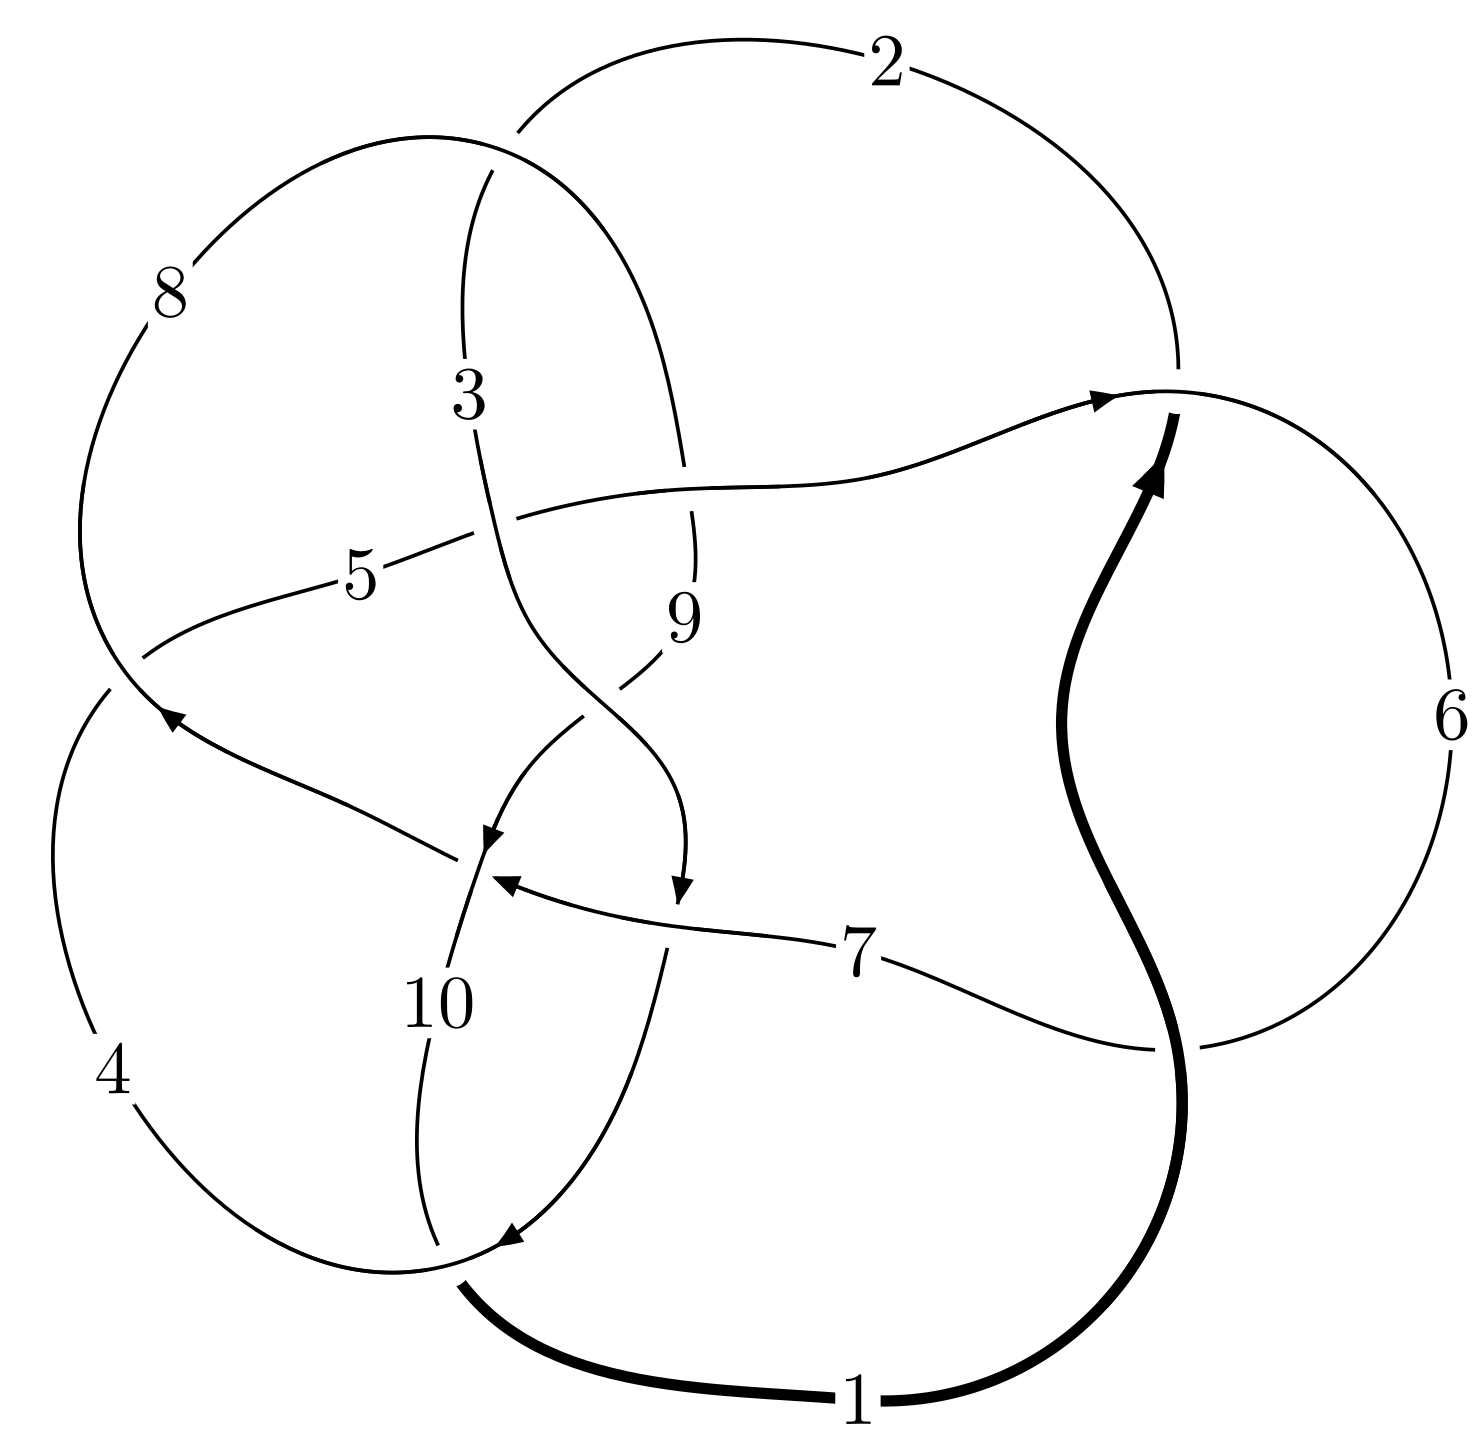
\includegraphics[width=112pt]{../../../GIT/diagram.site/Diagrams/png/248_10_164.png}\\
\ \ \ A knot diagram\footnotemark}&
\allowdisplaybreaks
\textbf{Linearized knot diagam} \\
\cline{2-2}
 &
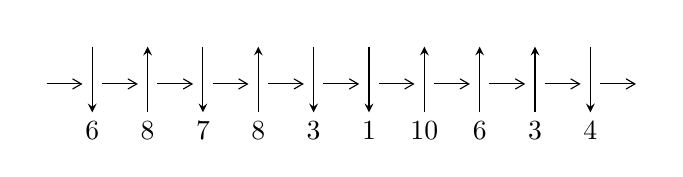
\begin{tikzpicture}[x=20pt, y=17pt]
	% nodes
	\node (C0) at (0, 0) {};
	\node (C1) at (1, 0) {};
	\node (C1U) at (1, +1) {};
	\node (C1D) at (1, -1) {6};

	\node (C2) at (2, 0) {};
	\node (C2U) at (2, +1) {};
	\node (C2D) at (2, -1) {8};

	\node (C3) at (3, 0) {};
	\node (C3U) at (3, +1) {};
	\node (C3D) at (3, -1) {7};

	\node (C4) at (4, 0) {};
	\node (C4U) at (4, +1) {};
	\node (C4D) at (4, -1) {8};

	\node (C5) at (5, 0) {};
	\node (C5U) at (5, +1) {};
	\node (C5D) at (5, -1) {3};

	\node (C6) at (6, 0) {};
	\node (C6U) at (6, +1) {};
	\node (C6D) at (6, -1) {1};

	\node (C7) at (7, 0) {};
	\node (C7U) at (7, +1) {};
	\node (C7D) at (7, -1) {10};

	\node (C8) at (8, 0) {};
	\node (C8U) at (8, +1) {};
	\node (C8D) at (8, -1) {6};

	\node (C9) at (9, 0) {};
	\node (C9U) at (9, +1) {};
	\node (C9D) at (9, -1) {3};

	\node (C10) at (10, 0) {};
	\node (C10U) at (10, +1) {};
	\node (C10D) at (10, -1) {4};
	\node (C11) at (11, 0) {};

	% arrows
	\draw[->,>={angle 60}]
	(C0) edge (C1) (C1) edge (C2) (C2) edge (C3) (C3) edge (C4) (C4) edge (C5) (C5) edge (C6) (C6) edge (C7) (C7) edge (C8) (C8) edge (C9) (C9) edge (C10) (C10) edge (C11) ;	\draw[->,>=stealth]
	(C1U) edge (C1D) (C2D) edge (C2U) (C3U) edge (C3D) (C4D) edge (C4U) (C5U) edge (C5D) (C6U) edge (C6D) (C7D) edge (C7U) (C8D) edge (C8U) (C9D) edge (C9U) (C10U) edge (C10D) ;
	\end{tikzpicture} \\
\hhline{~~} \\& 
\textbf{Solving Sequence} \\ \cline{2-2} 
 &
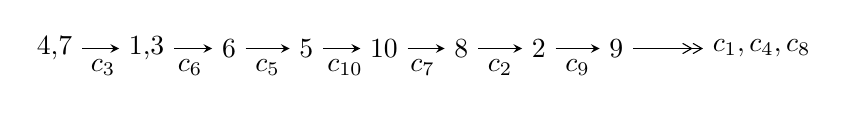
\begin{tikzpicture}[x=28pt, y=7pt]
	% node
	\node (A0) at (-1/8, 0) {4,7};
	\node (A1) at (17/16, 0) {1,3};
	\node (A2) at (17/8, 0) {6};
	\node (A3) at (25/8, 0) {5};
	\node (A4) at (33/8, 0) {10};
	\node (A5) at (41/8, 0) {8};
	\node (A6) at (49/8, 0) {2};
	\node (A7) at (57/8, 0) {9};
	\node (C1) at (1/2, -1) {$c_{3}$};
	\node (C2) at (13/8, -1) {$c_{6}$};
	\node (C3) at (21/8, -1) {$c_{5}$};
	\node (C4) at (29/8, -1) {$c_{10}$};
	\node (C5) at (37/8, -1) {$c_{7}$};
	\node (C6) at (45/8, -1) {$c_{2}$};
	\node (C7) at (53/8, -1) {$c_{9}$};
	\node (A8) at (9, 0) {$c_{1},c_{4},c_{8}$};

	% edge
	\draw[->,>=stealth]	
	(A0) edge (A1) (A1) edge (A2) (A2) edge (A3) (A3) edge (A4) (A4) edge (A5) (A5) edge (A6) (A6) edge (A7) ;
	\draw[->>,>={angle 60}]	
	(A7) edge (A8);
\end{tikzpicture} \\ 

\end{tabular} \\

\footnotetext{
The image of knot diagram is generated by the software ``\textbf{Draw programme}" developed by Andrew Bartholomew(\url{http://www.layer8.co.uk/maths/draw/index.htm\#Running-draw}), where we modified some parts for our purpose(\url{https://github.com/CATsTAILs/LinksPainter}).
}\phantom \\ \newline 
\centering \textbf{Ideals for irreducible components\footnotemark of $X_{\text{par}}$} 
 
\begin{align*}
I^u_{1}&=\langle 
b+u,\;-138 u^{11}+105 u^{10}+\cdots+142 a-155,\;u^{12}+u^9+6 u^8+u^7- u^6+2 u^5+5 u^4-2 u^3+2 u+1\rangle \\
I^u_{2}&=\langle 
22976741298 u^{15}-77906464811 u^{14}+\cdots+11233228513 b+21004036137,\\
\phantom{I^u_{2}}&\phantom{= \langle  }-2983129 u^{15}+13995185 u^{14}+\cdots+26682253 a-65290273,\;u^{16}-3 u^{15}+\cdots+4 u+1\rangle \\
I^u_{3}&=\langle 
b+u,\;3 u^5+u^4+2 u^3-3 u^2+2 a+6 u+1,\;u^6+u^4- u^3+3 u^2- u+1\rangle \\
\\
\end{align*}
\raggedright * 3 irreducible components of $\dim_{\mathbb{C}}=0$, with total 34 representations.\\
\footnotetext{All coefficients of polynomials are rational numbers. But the coefficients are sometimes approximated in decimal forms when there is not enough margin.}
\newpage
\renewcommand{\arraystretch}{1}
\centering \section*{I. $I^u_{1}= \langle b+u,\;-138 u^{11}+105 u^{10}+\cdots+142 a-155,\;u^{12}+u^9+\cdots+2 u+1 \rangle$}
\flushleft \textbf{(i) Arc colorings}\\
\begin{tabular}{m{7pt} m{180pt} m{7pt} m{180pt} }
\flushright $a_{4}=$&$\begin{pmatrix}1\\0\end{pmatrix}$ \\
\flushright $a_{7}=$&$\begin{pmatrix}0\\u\end{pmatrix}$ \\
\flushright $a_{1}=$&$\begin{pmatrix}0.971831 u^{11}-0.739437 u^{10}+\cdots+3.60563 u+1.09155\\- u\end{pmatrix}$ \\
\flushright $a_{3}=$&$\begin{pmatrix}1\\- u^2\end{pmatrix}$ \\
\flushright $a_{6}=$&$\begin{pmatrix}1.44718 u^{11}-0.0739437 u^{10}+\cdots+1.01056 u+3.60915\\-0.464789 u^{11}+0.0492958 u^{10}+\cdots+0.492958 u-0.739437\end{pmatrix}$ \\
\flushright $a_{5}=$&$\begin{pmatrix}0.978873 u^{11}+0.0704225 u^{10}+\cdots+0.204225 u+2.94366\\-0.0669014 u^{11}-0.193662 u^{10}+\cdots+0.313380 u-0.595070\end{pmatrix}$ \\
\flushright $a_{10}=$&$\begin{pmatrix}0.971831 u^{11}-0.739437 u^{10}+\cdots+2.60563 u+1.09155\\- u\end{pmatrix}$ \\
\flushright $a_{8}=$&$\begin{pmatrix}0.517606 u^{11}+0.0246479 u^{10}+\cdots-0.00352113 u+2.13028\\-0.464789 u^{11}+0.0492958 u^{10}+\cdots+0.492958 u-0.739437\end{pmatrix}$ \\
\flushright $a_{2}=$&$\begin{pmatrix}0.0422535 u^{11}+0.359155 u^{10}+\cdots-0.408451 u-0.387324\\0.468310 u^{11}-0.144366 u^{10}+\cdots+0.806338 u+0.665493\end{pmatrix}$ \\
\flushright $a_{9}=$&$\begin{pmatrix}0.507042 u^{11}-0.690141 u^{10}+\cdots+3.09859 u+0.352113\\-0.169014 u^{11}+0.0633803 u^{10}+\cdots-1.36620 u+0.0492958\end{pmatrix}$\\&\end{tabular}
\flushleft \textbf{(ii) Obstruction class $= -1$}\\~\\
\flushleft \textbf{(iii) Cusp Shapes $= -\frac{72}{71} u^{11}+\frac{169}{71} u^{10}-\frac{19}{71} u^9-\frac{56}{71} u^8-\frac{340}{71} u^7+\frac{943}{71} u^6+\frac{100}{71} u^5-\frac{288}{71} u^4-\frac{394}{71} u^3+\frac{984}{71} u^2-\frac{369}{71} u-\frac{192}{71}$}\\~\\
\newpage\renewcommand{\arraystretch}{1}
\flushleft \textbf{(iv) u-Polynomials at the component}\newline \\
\begin{tabular}{m{50pt}|m{274pt}}
Crossings & \hspace{64pt}u-Polynomials at each crossing \\
\hline $$\begin{aligned}c_{1},c_{6}\end{aligned}$$&$\begin{aligned}
&u^{12}+8 u^{11}+\cdots+96 u+16
\end{aligned}$\\
\hline $$\begin{aligned}c_{2},c_{8}\end{aligned}$$&$\begin{aligned}
&u^{12}- u^{11}+\cdots-2 u+1
\end{aligned}$\\
\hline $$\begin{aligned}c_{3},c_{10}\end{aligned}$$&$\begin{aligned}
&u^{12}- u^9+6 u^8- u^7- u^6-2 u^5+5 u^4+2 u^3-2 u+1
\end{aligned}$\\
\hline $$\begin{aligned}c_{4},c_{9}\end{aligned}$$&$\begin{aligned}
&u^{12}- u^{11}+\cdots+4 u^2+2
\end{aligned}$\\
\hline $$\begin{aligned}c_{5}\end{aligned}$$&$\begin{aligned}
&u^{12}-9 u^{11}+\cdots-20 u+16
\end{aligned}$\\
\hline $$\begin{aligned}c_{7}\end{aligned}$$&$\begin{aligned}
&u^{12}+8 u^{11}+\cdots+22 u+4
\end{aligned}$\\
\hline
\end{tabular}\\~\\
\newpage\renewcommand{\arraystretch}{1}
\flushleft \textbf{(v) Riley Polynomials at the component}\newline \\
\begin{tabular}{m{50pt}|m{274pt}}
Crossings & \hspace{64pt}Riley Polynomials at each crossing \\
\hline $$\begin{aligned}c_{1},c_{6}\end{aligned}$$&$\begin{aligned}
&y^{12}+6 y^{11}+\cdots-640 y+256
\end{aligned}$\\
\hline $$\begin{aligned}c_{2},c_{8}\end{aligned}$$&$\begin{aligned}
&y^{12}+17 y^{11}+\cdots+6 y+1
\end{aligned}$\\
\hline $$\begin{aligned}c_{3},c_{10}\end{aligned}$$&$\begin{aligned}
&y^{12}+12 y^{10}+\cdots-4 y+1
\end{aligned}$\\
\hline $$\begin{aligned}c_{4},c_{9}\end{aligned}$$&$\begin{aligned}
&y^{12}+5 y^{11}+\cdots+16 y+4
\end{aligned}$\\
\hline $$\begin{aligned}c_{5}\end{aligned}$$&$\begin{aligned}
&y^{12}-11 y^{11}+\cdots+80 y+256
\end{aligned}$\\
\hline $$\begin{aligned}c_{7}\end{aligned}$$&$\begin{aligned}
&y^{12}+2 y^{11}+\cdots+84 y+16
\end{aligned}$\\
\hline
\end{tabular}\\~\\
\newpage\flushleft \textbf{(vi) Complex Volumes and Cusp Shapes}
$$\begin{array}{c|c|c}  
\text{Solutions to }I^u_{1}& \I (\text{vol} + \sqrt{-1}CS) & \text{Cusp shape}\\
 \hline 
\begin{aligned}
u &= \phantom{-}0.433167 + 0.820343 I \\
a &= \phantom{-}1.77573 - 0.27759 I \\
b &= -0.433167 - 0.820343 I\end{aligned}
 & -2.63922 - 4.58392 I & \phantom{-}1.89423 + 6.22117 I \\ \hline\begin{aligned}
u &= \phantom{-}0.433167 - 0.820343 I \\
a &= \phantom{-}1.77573 + 0.27759 I \\
b &= -0.433167 + 0.820343 I\end{aligned}
 & -2.63922 + 4.58392 I & \phantom{-}1.89423 - 6.22117 I \\ \hline\begin{aligned}
u &= -0.894529 + 0.606911 I \\
a &= -0.948486 - 0.965514 I \\
b &= \phantom{-}0.894529 - 0.606911 I\end{aligned}
 & -7.98844 + 5.04592 I & -3.50212 - 4.93530 I \\ \hline\begin{aligned}
u &= -0.894529 - 0.606911 I \\
a &= -0.948486 + 0.965514 I \\
b &= \phantom{-}0.894529 + 0.606911 I\end{aligned}
 & -7.98844 - 5.04592 I & -3.50212 + 4.93530 I \\ \hline\begin{aligned}
u &= \phantom{-}0.727666 + 0.459131 I \\
a &= \phantom{-}0.686537 - 0.236758 I \\
b &= -0.727666 - 0.459131 I\end{aligned}
 & -1.29616 - 0.86105 I & -4.70470 + 1.78151 I \\ \hline\begin{aligned}
u &= \phantom{-}0.727666 - 0.459131 I \\
a &= \phantom{-}0.686537 + 0.236758 I \\
b &= -0.727666 + 0.459131 I\end{aligned}
 & -1.29616 + 0.86105 I & -4.70470 - 1.78151 I \\ \hline\begin{aligned}
u &= -0.925706 + 1.050550 I \\
a &= -0.840738 + 0.491457 I \\
b &= \phantom{-}0.925706 - 1.050550 I\end{aligned}
 & \phantom{-}3.38867 + 4.08003 I & -1.46265 - 0.78652 I \\ \hline\begin{aligned}
u &= -0.925706 - 1.050550 I \\
a &= -0.840738 - 0.491457 I \\
b &= \phantom{-}0.925706 + 1.050550 I\end{aligned}
 & \phantom{-}3.38867 - 4.08003 I & -1.46265 + 0.78652 I \\ \hline\begin{aligned}
u &= -0.444254 + 0.260304 I \\
a &= -1.11367 + 2.11911 I \\
b &= \phantom{-}0.444254 - 0.260304 I\end{aligned}
 & \phantom{-}1.58084 + 1.46904 I & \phantom{-}1.29817 - 5.01402 I \\ \hline\begin{aligned}
u &= -0.444254 - 0.260304 I \\
a &= -1.11367 - 2.11911 I \\
b &= \phantom{-}0.444254 + 0.260304 I\end{aligned}
 & \phantom{-}1.58084 - 1.46904 I & \phantom{-}1.29817 + 5.01402 I\\
 \hline 
 \end{array}$$\newpage$$\begin{array}{c|c|c}  
\text{Solutions to }I^u_{1}& \I (\text{vol} + \sqrt{-1}CS) & \text{Cusp shape}\\
 \hline 
\begin{aligned}
u &= \phantom{-}1.10366 + 1.16882 I \\
a &= \phantom{-}0.940626 + 0.241992 I \\
b &= -1.10366 - 1.16882 I\end{aligned}
 & -4.56023 - 12.50670 I & -0.52291 + 6.78913 I \\ \hline\begin{aligned}
u &= \phantom{-}1.10366 - 1.16882 I \\
a &= \phantom{-}0.940626 - 0.241992 I \\
b &= -1.10366 + 1.16882 I\end{aligned}
 & -4.56023 + 12.50670 I & -0.52291 - 6.78913 I\\
 \hline 
 \end{array}$$\newpage\newpage\renewcommand{\arraystretch}{1}
\centering \section*{II. $I^u_{2}= \langle 2.30\times10^{10} u^{15}-7.79\times10^{10} u^{14}+\cdots+1.12\times10^{10} b+2.10\times10^{10},\;-2.98\times10^{6} u^{15}+1.40\times10^{7} u^{14}+\cdots+2.67\times10^{7} a-6.53\times10^{7},\;u^{16}-3 u^{15}+\cdots+4 u+1 \rangle$}
\flushleft \textbf{(i) Arc colorings}\\
\begin{tabular}{m{7pt} m{180pt} m{7pt} m{180pt} }
\flushright $a_{4}=$&$\begin{pmatrix}1\\0\end{pmatrix}$ \\
\flushright $a_{7}=$&$\begin{pmatrix}0\\u\end{pmatrix}$ \\
\flushright $a_{1}=$&$\begin{pmatrix}0.111802 u^{15}-0.524513 u^{14}+\cdots-0.695051 u+2.44696\\-2.04543 u^{15}+6.93536 u^{14}+\cdots-10.9045 u-1.86981\end{pmatrix}$ \\
\flushright $a_{3}=$&$\begin{pmatrix}1\\- u^2\end{pmatrix}$ \\
\flushright $a_{6}=$&$\begin{pmatrix}0.888198 u^{15}-2.47549 u^{14}+\cdots+12.6951 u+1.55304\\1.45142 u^{15}-4.13944 u^{14}+\cdots+13.6179 u+4.66725\end{pmatrix}$ \\
\flushright $a_{5}=$&$\begin{pmatrix}2.23464 u^{15}-6.47872 u^{14}+\cdots+24.6683 u+6.03118\\1.68993 u^{15}-4.95565 u^{14}+\cdots+15.1088 u+4.70335\end{pmatrix}$ \\
\flushright $a_{10}=$&$\begin{pmatrix}-1.93362 u^{15}+6.41085 u^{14}+\cdots-11.5996 u+0.577142\\-2.04543 u^{15}+6.93536 u^{14}+\cdots-10.9045 u-1.86981\end{pmatrix}$ \\
\flushright $a_{8}=$&$\begin{pmatrix}2.50110 u^{15}-6.52849 u^{14}+\cdots+28.7759 u+8.29535\\0.161484 u^{15}+0.0864436 u^{14}+\cdots+4.46296 u+2.07506\end{pmatrix}$ \\
\flushright $a_{2}=$&$\begin{pmatrix}-0.888198 u^{15}+2.47549 u^{14}+\cdots-12.6951 u-1.55304\\-1.34644 u^{15}+4.00323 u^{14}+\cdots-11.9733 u-4.47814\end{pmatrix}$ \\
\flushright $a_{9}=$&$\begin{pmatrix}0.0729519 u^{15}-0.441341 u^{14}+\cdots-0.188785 u+3.05693\\-2.21877 u^{15}+7.30458 u^{14}+\cdots-12.2278 u-2.70227\end{pmatrix}$\\&\end{tabular}
\flushleft \textbf{(ii) Obstruction class $= -1$}\\~\\
\flushleft \textbf{(iii) Cusp Shapes $= -\frac{62712632292}{11233228513} u^{15}+\frac{222551627880}{11233228513} u^{14}+\cdots-\frac{386527091664}{11233228513} u-\frac{36877222054}{11233228513}$}\\~\\
\newpage\renewcommand{\arraystretch}{1}
\flushleft \textbf{(iv) u-Polynomials at the component}\newline \\
\begin{tabular}{m{50pt}|m{274pt}}
Crossings & \hspace{64pt}u-Polynomials at each crossing \\
\hline $$\begin{aligned}c_{1},c_{6}\end{aligned}$$&$\begin{aligned}
&(u^2- u+1)^8
\end{aligned}$\\
\hline $$\begin{aligned}c_{2},c_{8}\end{aligned}$$&$\begin{aligned}
&u^{16}+u^{15}+\cdots-48 u+19
\end{aligned}$\\
\hline $$\begin{aligned}c_{3},c_{10}\end{aligned}$$&$\begin{aligned}
&u^{16}+3 u^{15}+\cdots-4 u+1
\end{aligned}$\\
\hline $$\begin{aligned}c_{4},c_{9}\end{aligned}$$&$\begin{aligned}
&u^{16}+u^{15}+\cdots-6 u+1
\end{aligned}$\\
\hline $$\begin{aligned}c_{5}\end{aligned}$$&$\begin{aligned}
&(u^4+3 u^3+u^2-2 u+1)^4
\end{aligned}$\\
\hline $$\begin{aligned}c_{7}\end{aligned}$$&$\begin{aligned}
&(u^4- u^3+u^2+1)^4
\end{aligned}$\\
\hline
\end{tabular}\\~\\
\newpage\renewcommand{\arraystretch}{1}
\flushleft \textbf{(v) Riley Polynomials at the component}\newline \\
\begin{tabular}{m{50pt}|m{274pt}}
Crossings & \hspace{64pt}Riley Polynomials at each crossing \\
\hline $$\begin{aligned}c_{1},c_{6}\end{aligned}$$&$\begin{aligned}
&(y^2+y+1)^8
\end{aligned}$\\
\hline $$\begin{aligned}c_{2},c_{8}\end{aligned}$$&$\begin{aligned}
&y^{16}+15 y^{15}+\cdots+2332 y+361
\end{aligned}$\\
\hline $$\begin{aligned}c_{3},c_{10}\end{aligned}$$&$\begin{aligned}
&y^{16}+3 y^{15}+\cdots+8 y+1
\end{aligned}$\\
\hline $$\begin{aligned}c_{4},c_{9}\end{aligned}$$&$\begin{aligned}
&y^{16}+7 y^{15}+\cdots+134 y+1
\end{aligned}$\\
\hline $$\begin{aligned}c_{5}\end{aligned}$$&$\begin{aligned}
&(y^4-7 y^3+15 y^2-2 y+1)^4
\end{aligned}$\\
\hline $$\begin{aligned}c_{7}\end{aligned}$$&$\begin{aligned}
&(y^4+y^3+3 y^2+2 y+1)^4
\end{aligned}$\\
\hline
\end{tabular}\\~\\
\newpage\flushleft \textbf{(vi) Complex Volumes and Cusp Shapes}
$$\begin{array}{c|c|c}  
\text{Solutions to }I^u_{2}& \I (\text{vol} + \sqrt{-1}CS) & \text{Cusp shape}\\
 \hline 
\begin{aligned}
u &= \phantom{-}1.051690 + 0.235939 I \\
a &= -0.276759 + 0.885546 I \\
b &= \phantom{-}0.44895 - 1.60911 I\end{aligned}
 & -5.14581 + 0.61478 I & -3.82674 + 1.44464 I \\ \hline\begin{aligned}
u &= \phantom{-}1.051690 - 0.235939 I \\
a &= -0.276759 - 0.885546 I \\
b &= \phantom{-}0.44895 + 1.60911 I\end{aligned}
 & -5.14581 - 0.61478 I & -3.82674 - 1.44464 I \\ \hline\begin{aligned}
u &= -0.804589 + 0.808792 I \\
a &= \phantom{-}0.847270 - 0.224662 I \\
b &= -0.88699 + 1.31736 I\end{aligned}
 & \phantom{-}1.85594 + 5.19385 I & -0.17326 - 6.02890 I \\ \hline\begin{aligned}
u &= -0.804589 - 0.808792 I \\
a &= \phantom{-}0.847270 + 0.224662 I \\
b &= -0.88699 - 1.31736 I\end{aligned}
 & \phantom{-}1.85594 - 5.19385 I & -0.17326 + 6.02890 I \\ \hline\begin{aligned}
u &= -0.321200 + 0.647019 I \\
a &= -0.766065 + 1.153070 I \\
b &= \phantom{-}0.160429 + 0.464095 I\end{aligned}
 & \phantom{-}1.85594 + 1.13408 I & -0.173262 + 0.899303 I \\ \hline\begin{aligned}
u &= -0.321200 - 0.647019 I \\
a &= -0.766065 - 1.153070 I \\
b &= \phantom{-}0.160429 - 0.464095 I\end{aligned}
 & \phantom{-}1.85594 - 1.13408 I & -0.173262 - 0.899303 I \\ \hline\begin{aligned}
u &= -0.160429 + 0.464095 I \\
a &= \phantom{-}1.99954 + 0.38616 I \\
b &= \phantom{-}0.321200 + 0.647019 I\end{aligned}
 & \phantom{-}1.85594 - 1.13408 I & -0.173262 - 0.899303 I \\ \hline\begin{aligned}
u &= -0.160429 - 0.464095 I \\
a &= \phantom{-}1.99954 - 0.38616 I \\
b &= \phantom{-}0.321200 - 0.647019 I\end{aligned}
 & \phantom{-}1.85594 + 1.13408 I & -0.173262 + 0.899303 I \\ \hline\begin{aligned}
u &= -0.311042 + 0.310121 I \\
a &= \phantom{-}2.19827 - 0.59252 I \\
b &= -1.60753 - 1.13440 I\end{aligned}
 & -5.14581 + 3.44499 I & -3.82674 - 8.37284 I \\ \hline\begin{aligned}
u &= -0.311042 - 0.310121 I \\
a &= \phantom{-}2.19827 + 0.59252 I \\
b &= -1.60753 + 1.13440 I\end{aligned}
 & -5.14581 - 3.44499 I & -3.82674 + 8.37284 I\\
 \hline 
 \end{array}$$\newpage$$\begin{array}{c|c|c}  
\text{Solutions to }I^u_{2}& \I (\text{vol} + \sqrt{-1}CS) & \text{Cusp shape}\\
 \hline 
\begin{aligned}
u &= \phantom{-}0.88699 + 1.31736 I \\
a &= -0.628172 - 0.043405 I \\
b &= \phantom{-}0.804589 + 0.808792 I\end{aligned}
 & \phantom{-}1.85594 - 5.19385 I & -0.17326 + 6.02890 I \\ \hline\begin{aligned}
u &= \phantom{-}0.88699 - 1.31736 I \\
a &= -0.628172 + 0.043405 I \\
b &= \phantom{-}0.804589 - 0.808792 I\end{aligned}
 & \phantom{-}1.85594 + 5.19385 I & -0.17326 - 6.02890 I \\ \hline\begin{aligned}
u &= -0.44895 + 1.60911 I \\
a &= \phantom{-}0.579766 + 0.148974 I \\
b &= -1.051690 - 0.235939 I\end{aligned}
 & -5.14581 + 0.61478 I & -3.82674 + 1.44464 I \\ \hline\begin{aligned}
u &= -0.44895 - 1.60911 I \\
a &= \phantom{-}0.579766 - 0.148974 I \\
b &= -1.051690 + 0.235939 I\end{aligned}
 & -5.14581 - 0.61478 I & -3.82674 - 1.44464 I \\ \hline\begin{aligned}
u &= \phantom{-}1.60753 + 1.13440 I \\
a &= \phantom{-}0.046151 + 0.506163 I \\
b &= \phantom{-}0.311042 - 0.310121 I\end{aligned}
 & -5.14581 + 3.44499 I & -3.82674 - 8.37284 I \\ \hline\begin{aligned}
u &= \phantom{-}1.60753 - 1.13440 I \\
a &= \phantom{-}0.046151 - 0.506163 I \\
b &= \phantom{-}0.311042 + 0.310121 I\end{aligned}
 & -5.14581 - 3.44499 I & -3.82674 + 8.37284 I\\
 \hline 
 \end{array}$$\newpage\newpage\renewcommand{\arraystretch}{1}
\centering \section*{III. $I^u_{3}= \langle b+u,\;3 u^5+u^4+2 u^3-3 u^2+2 a+6 u+1,\;u^6+u^4- u^3+3 u^2- u+1 \rangle$}
\flushleft \textbf{(i) Arc colorings}\\
\begin{tabular}{m{7pt} m{180pt} m{7pt} m{180pt} }
\flushright $a_{4}=$&$\begin{pmatrix}1\\0\end{pmatrix}$ \\
\flushright $a_{7}=$&$\begin{pmatrix}0\\u\end{pmatrix}$ \\
\flushright $a_{1}=$&$\begin{pmatrix}-\frac{3}{2} u^5-\frac{1}{2} u^4+\cdots-3 u-\frac{1}{2}\\- u\end{pmatrix}$ \\
\flushright $a_{3}=$&$\begin{pmatrix}1\\- u^2\end{pmatrix}$ \\
\flushright $a_{6}=$&$\begin{pmatrix}- u^4- u^2+u-3\\-\frac{1}{2} u^5-\frac{1}{2} u^4- u^3+\frac{1}{2} u^2-\frac{1}{2}\end{pmatrix}$ \\
\flushright $a_{5}=$&$\begin{pmatrix}-\frac{1}{2} u^5-\frac{3}{2} u^4- u^3-\frac{1}{2} u^2-\frac{5}{2}\\- u^4- u^3- u^2-1\end{pmatrix}$ \\
\flushright $a_{10}=$&$\begin{pmatrix}-\frac{3}{2} u^5-\frac{1}{2} u^4+\cdots-4 u-\frac{1}{2}\\- u\end{pmatrix}$ \\
\flushright $a_{8}=$&$\begin{pmatrix}- u^5-2 u^4- u^3- u-4\\-\frac{1}{2} u^5-\frac{1}{2} u^4+\frac{1}{2} u^2-\frac{1}{2}\end{pmatrix}$ \\
\flushright $a_{2}=$&$\begin{pmatrix}\frac{1}{2} u^5-\frac{3}{2} u^4-\frac{3}{2} u^2+3 u-\frac{7}{2}\\\frac{1}{2} u^5+\frac{1}{2} u^4+\cdots+u-\frac{1}{2}\end{pmatrix}$ \\
\flushright $a_{9}=$&$\begin{pmatrix}-2 u^5- u^4- u^3+2 u^2-4 u-1\\-\frac{1}{2} u^5-\frac{1}{2} u^4+\cdots- u-\frac{1}{2}\end{pmatrix}$\\&\end{tabular}
\flushleft \textbf{(ii) Obstruction class $= 1$}\\~\\
\flushleft \textbf{(iii) Cusp Shapes $= 7 u^5+5 u^4+6 u^3-3 u^2+11 u+10$}\\~\\
\newpage\renewcommand{\arraystretch}{1}
\flushleft \textbf{(iv) u-Polynomials at the component}\newline \\
\begin{tabular}{m{50pt}|m{274pt}}
Crossings & \hspace{64pt}u-Polynomials at each crossing \\
\hline $$\begin{aligned}c_{1}\end{aligned}$$&$\begin{aligned}
&u^6- u^5+3 u^4- u^3+3 u^2+2
\end{aligned}$\\
\hline $$\begin{aligned}c_{2},c_{8}\end{aligned}$$&$\begin{aligned}
&u^6- u^5+2 u^4-2 u^2+u+1
\end{aligned}$\\
\hline $$\begin{aligned}c_{3},c_{10}\end{aligned}$$&$\begin{aligned}
&u^6+u^4- u^3+3 u^2- u+1
\end{aligned}$\\
\hline $$\begin{aligned}c_{4},c_{9}\end{aligned}$$&$\begin{aligned}
&u^6- u^5+2 u^4+2 u^3- u^2+2 u+2
\end{aligned}$\\
\hline $$\begin{aligned}c_{5}\end{aligned}$$&$\begin{aligned}
&u^6+4 u^5+6 u^4+8 u^3+10 u^2+4 u+1
\end{aligned}$\\
\hline $$\begin{aligned}c_{6}\end{aligned}$$&$\begin{aligned}
&u^6+u^5+3 u^4+u^3+3 u^2+2
\end{aligned}$\\
\hline $$\begin{aligned}c_{7}\end{aligned}$$&$\begin{aligned}
&u^6+3 u^5+5 u^4+3 u^3+u^2+1
\end{aligned}$\\
\hline
\end{tabular}\\~\\
\newpage\renewcommand{\arraystretch}{1}
\flushleft \textbf{(v) Riley Polynomials at the component}\newline \\
\begin{tabular}{m{50pt}|m{274pt}}
Crossings & \hspace{64pt}Riley Polynomials at each crossing \\
\hline $$\begin{aligned}c_{1},c_{6}\end{aligned}$$&$\begin{aligned}
&y^6+5 y^5+13 y^4+21 y^3+21 y^2+12 y+4
\end{aligned}$\\
\hline $$\begin{aligned}c_{2},c_{8}\end{aligned}$$&$\begin{aligned}
&y^6+3 y^5-4 y^3+8 y^2-5 y+1
\end{aligned}$\\
\hline $$\begin{aligned}c_{3},c_{10}\end{aligned}$$&$\begin{aligned}
&y^6+2 y^5+7 y^4+7 y^3+9 y^2+5 y+1
\end{aligned}$\\
\hline $$\begin{aligned}c_{4},c_{9}\end{aligned}$$&$\begin{aligned}
&y^6+3 y^5+6 y^4+y^2-8 y+4
\end{aligned}$\\
\hline $$\begin{aligned}c_{5}\end{aligned}$$&$\begin{aligned}
&y^6-4 y^5-8 y^4+26 y^3+48 y^2+4 y+1
\end{aligned}$\\
\hline $$\begin{aligned}c_{7}\end{aligned}$$&$\begin{aligned}
&y^6+y^5+9 y^4+3 y^3+11 y^2+2 y+1
\end{aligned}$\\
\hline
\end{tabular}\\~\\
\newpage\flushleft \textbf{(vi) Complex Volumes and Cusp Shapes}
$$\begin{array}{c|c|c}  
\text{Solutions to }I^u_{3}& \I (\text{vol} + \sqrt{-1}CS) & \text{Cusp shape}\\
 \hline 
\begin{aligned}
u &= \phantom{-}0.747107 + 0.813589 I \\
a &= \phantom{-}0.239424 + 0.758194 I \\
b &= -0.747107 - 0.813589 I\end{aligned}
 & -4.92982 + 2.38212 I & -1.44137 - 0.69060 I \\ \hline\begin{aligned}
u &= \phantom{-}0.747107 - 0.813589 I \\
a &= \phantom{-}0.239424 - 0.758194 I \\
b &= -0.747107 + 0.813589 I\end{aligned}
 & -4.92982 - 2.38212 I & -1.44137 + 0.69060 I \\ \hline\begin{aligned}
u &= \phantom{-}0.125253 + 0.619808 I \\
a &= -1.46927 - 1.44270 I \\
b &= -0.125253 - 0.619808 I\end{aligned}
 & \phantom{-}2.50509 - 1.44331 I & \phantom{-}12.78155 + 4.91052 I \\ \hline\begin{aligned}
u &= \phantom{-}0.125253 - 0.619808 I \\
a &= -1.46927 + 1.44270 I \\
b &= -0.125253 + 0.619808 I\end{aligned}
 & \phantom{-}2.50509 + 1.44331 I & \phantom{-}12.78155 - 4.91052 I \\ \hline\begin{aligned}
u &= -0.87236 + 1.13524 I \\
a &= -0.770152 + 0.391132 I \\
b &= \phantom{-}0.87236 - 1.13524 I\end{aligned}
 & \phantom{-}4.06966 + 4.74338 I & \phantom{-}5.65982 - 6.07362 I \\ \hline\begin{aligned}
u &= -0.87236 - 1.13524 I \\
a &= -0.770152 - 0.391132 I \\
b &= \phantom{-}0.87236 + 1.13524 I\end{aligned}
 & \phantom{-}4.06966 - 4.74338 I & \phantom{-}5.65982 + 6.07362 I\\
 \hline 
 \end{array}$$\newpage
\newpage\renewcommand{\arraystretch}{1}
\centering \section*{ IV. u-Polynomials}
\begin{tabular}{m{50pt}|m{274pt}}
Crossings & \hspace{64pt}u-Polynomials at each crossing \\
\hline $$\begin{aligned}c_{1}\end{aligned}$$&$\begin{aligned}
&((u^2- u+1)^8)(u^6- u^5+\cdots+3 u^2+2)(u^{12}+8 u^{11}+\cdots+96 u+16)
\end{aligned}$\\
\hline $$\begin{aligned}c_{2},c_{8}\end{aligned}$$&$\begin{aligned}
&(u^6- u^5+2 u^4-2 u^2+u+1)(u^{12}- u^{11}+\cdots-2 u+1)\\
&\cdot(u^{16}+u^{15}+\cdots-48 u+19)
\end{aligned}$\\
\hline $$\begin{aligned}c_{3},c_{10}\end{aligned}$$&$\begin{aligned}
&(u^6+u^4- u^3+3 u^2- u+1)\\
&\cdot(u^{12}- u^9+6 u^8- u^7- u^6-2 u^5+5 u^4+2 u^3-2 u+1)\\
&\cdot(u^{16}+3 u^{15}+\cdots-4 u+1)
\end{aligned}$\\
\hline $$\begin{aligned}c_{4},c_{9}\end{aligned}$$&$\begin{aligned}
&(u^6- u^5+2 u^4+2 u^3- u^2+2 u+2)(u^{12}- u^{11}+\cdots+4 u^2+2)\\
&\cdot(u^{16}+u^{15}+\cdots-6 u+1)
\end{aligned}$\\
\hline $$\begin{aligned}c_{5}\end{aligned}$$&$\begin{aligned}
&(u^4+3 u^3+u^2-2 u+1)^4(u^6+4 u^5+6 u^4+8 u^3+10 u^2+4 u+1)\\
&\cdot(u^{12}-9 u^{11}+\cdots-20 u+16)
\end{aligned}$\\
\hline $$\begin{aligned}c_{6}\end{aligned}$$&$\begin{aligned}
&((u^2- u+1)^8)(u^6+u^5+\cdots+3 u^2+2)(u^{12}+8 u^{11}+\cdots+96 u+16)
\end{aligned}$\\
\hline $$\begin{aligned}c_{7}\end{aligned}$$&$\begin{aligned}
&(u^4- u^3+u^2+1)^4(u^6+3 u^5+5 u^4+3 u^3+u^2+1)\\
&\cdot(u^{12}+8 u^{11}+\cdots+22 u+4)
\end{aligned}$\\
\hline
\end{tabular}\newpage\renewcommand{\arraystretch}{1}
\centering \section*{ V. Riley Polynomials}
\begin{tabular}{m{50pt}|m{274pt}}
Crossings & \hspace{64pt}Riley Polynomials at each crossing \\
\hline $$\begin{aligned}c_{1},c_{6}\end{aligned}$$&$\begin{aligned}
&(y^2+y+1)^8(y^6+5 y^5+13 y^4+21 y^3+21 y^2+12 y+4)\\
&\cdot(y^{12}+6 y^{11}+\cdots-640 y+256)
\end{aligned}$\\
\hline $$\begin{aligned}c_{2},c_{8}\end{aligned}$$&$\begin{aligned}
&(y^6+3 y^5-4 y^3+8 y^2-5 y+1)(y^{12}+17 y^{11}+\cdots+6 y+1)\\
&\cdot(y^{16}+15 y^{15}+\cdots+2332 y+361)
\end{aligned}$\\
\hline $$\begin{aligned}c_{3},c_{10}\end{aligned}$$&$\begin{aligned}
&(y^6+2 y^5+\cdots+5 y+1)(y^{12}+12 y^{10}+\cdots-4 y+1)\\
&\cdot(y^{16}+3 y^{15}+\cdots+8 y+1)
\end{aligned}$\\
\hline $$\begin{aligned}c_{4},c_{9}\end{aligned}$$&$\begin{aligned}
&(y^6+3 y^5+6 y^4+y^2-8 y+4)(y^{12}+5 y^{11}+\cdots+16 y+4)\\
&\cdot(y^{16}+7 y^{15}+\cdots+134 y+1)
\end{aligned}$\\
\hline $$\begin{aligned}c_{5}\end{aligned}$$&$\begin{aligned}
&((y^4-7 y^3+15 y^2-2 y+1)^4)(y^6-4 y^5+\cdots+4 y+1)\\
&\cdot(y^{12}-11 y^{11}+\cdots+80 y+256)
\end{aligned}$\\
\hline $$\begin{aligned}c_{7}\end{aligned}$$&$\begin{aligned}
&(y^4+y^3+3 y^2+2 y+1)^4(y^6+y^5+9 y^4+3 y^3+11 y^2+2 y+1)\\
&\cdot(y^{12}+2 y^{11}+\cdots+84 y+16)
\end{aligned}$\\
\hline
\end{tabular}
\vskip 2pc
\end{document}